\chapter{Conclusão}

\section{Trabalhos Futuros}
O presente trabalho consiste na primeira etapa de um estudo realizado em 2 semestres. Para a segunda etapa do Trabalho de Conclusão de Curso espera-se implementar algumas funcionalidades adicionais para aumentar o escopo do projeto:
\begin{itemize}
    \item Envio de dados em tempo real para a central;
    \item Utilização do bando de dados HDF para armazenar dados númericos em alta performance;
    \item Criação de \textit{managers} para extrair mensagens não enviadas para o servidor;
    \item Permitir registro de transdutores para cada campus da Universidade;
    \item Calcular médias mensais, semanais e diárias utilizando os pacotes \textit{numpy} e {pandas};
    \item Gerar relatórios que supram as necessidades específicas do projeto.
\end{itemize}

\section{Cronograma}
Para a realização do cronograma do projeto, figura \ref{cronograma}, utilizou-se a ferramenta \textit{Gantter}. Esta ferramenta aborda como dividiram-se as sprints e atividades realizadas no decorrer do desenvolvimento do SME-UnB.

\begin{figure}[!htpb]
    \centering
    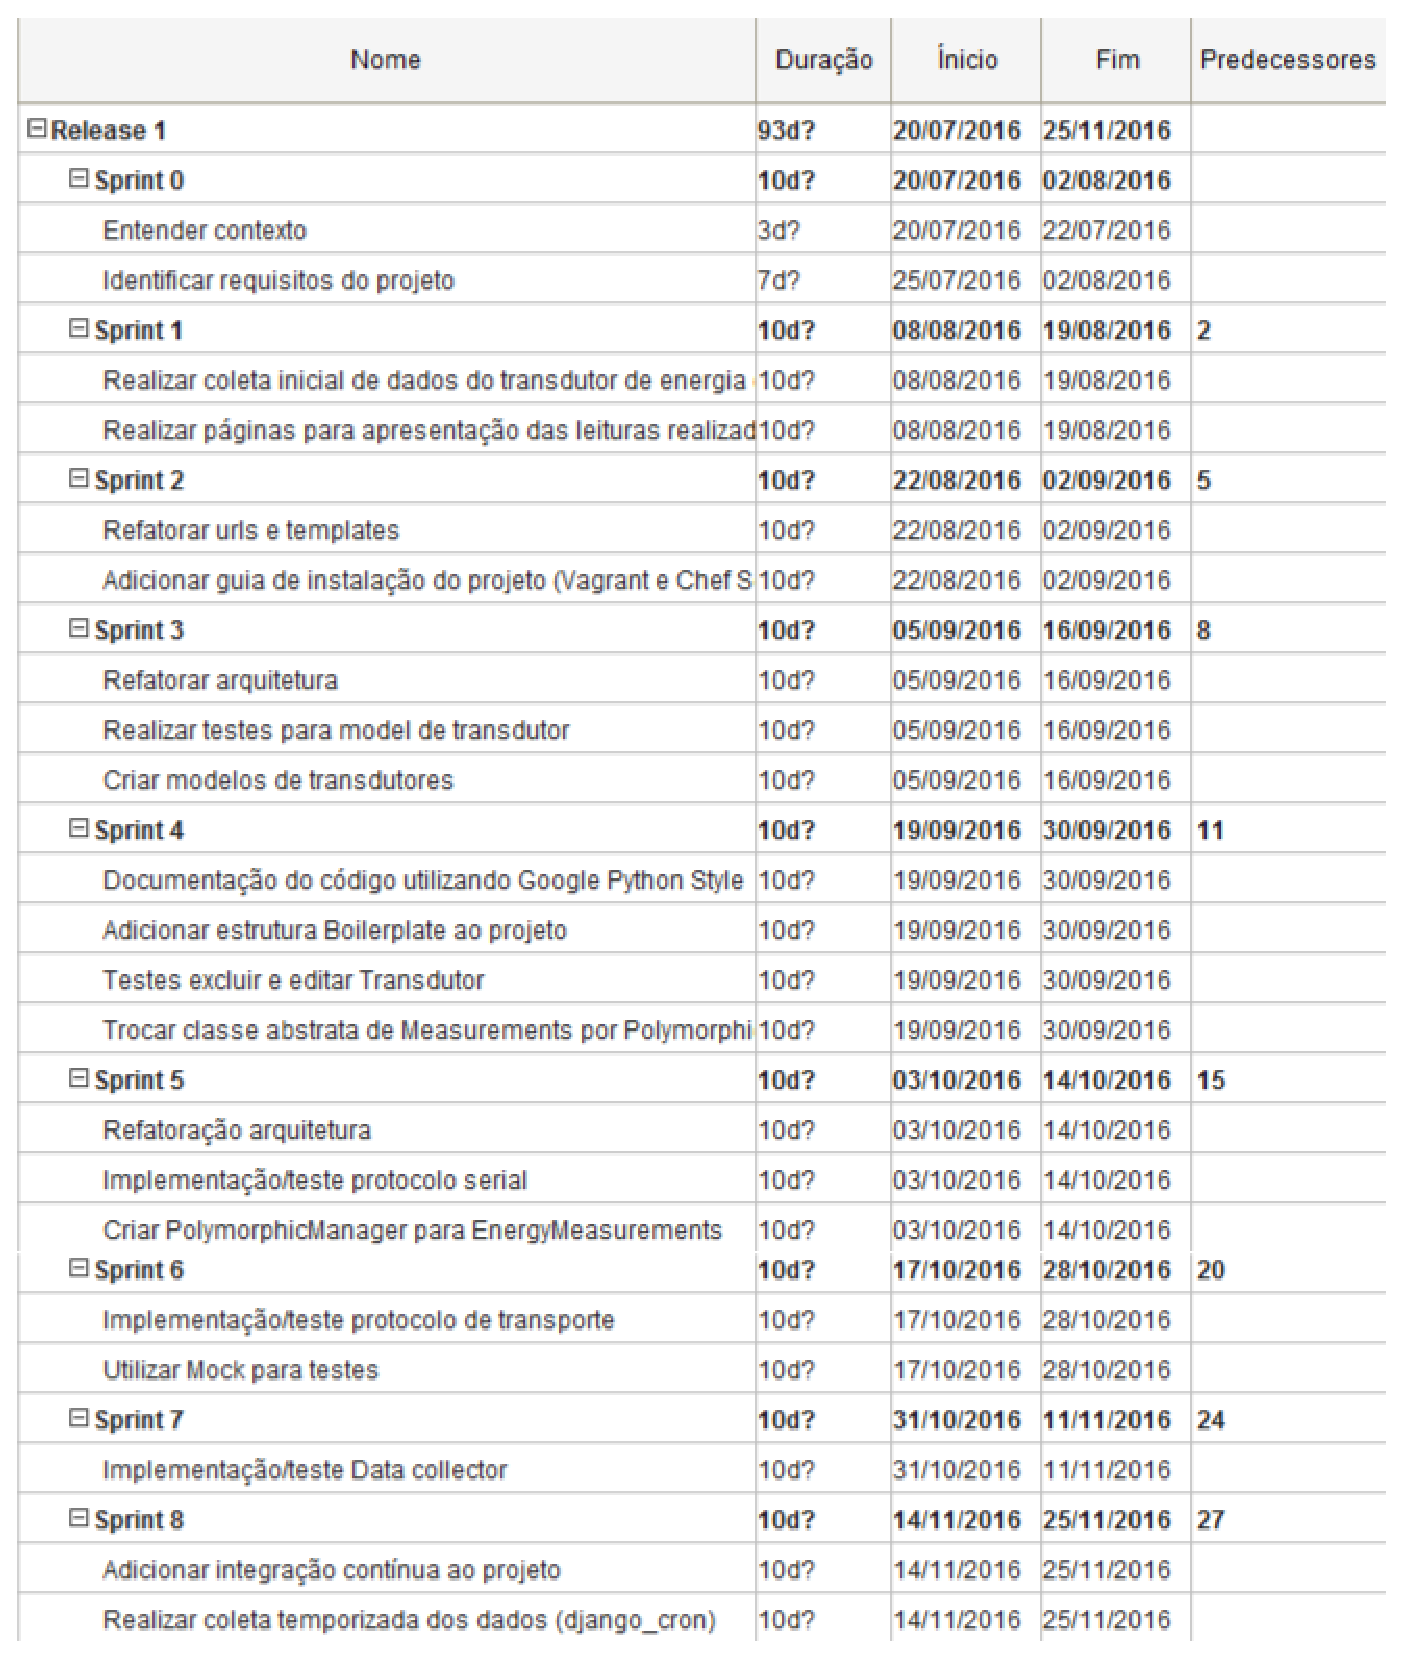
\includegraphics[keepaspectratio=true,scale=0.5]{figuras/cronograma.eps}
    \caption{Cronograma do Projeto.}
    \label{cronograma}
\end{figure}